\documentclass[12pt]{article}
\usepackage[switch, modulo]{lineno}
\usepackage[utf8]{inputenc}
\usepackage{amsmath}
\usepackage{amsfonts}
\usepackage{amssymb}
\usepackage{bm}
\usepackage{graphicx}
\usepackage{cite}
\usepackage{tabularx}
\usepackage{subfig}
\usepackage{listings}
\usepackage{courier}
\usepackage{booktabs}
\usepackage{abstract,lipsum}
\usepackage{soul}

\usepackage{upgreek} %%% This package provides non-italic greek letters: \upalpha, \upbeta or \Upalpha, \Upbeta for uppercase.

\usepackage{algorithm}
\usepackage{algpseudocode}
\makeatletter
\def\BState{\State\hskip-\ALG@thistlm}
\makeatother

\newcommand{\tabitem}{~~\llap{\textbullet}~~}

\newcolumntype{L}[1]{>{\raggedright\arraybackslash}X}%
\newcolumntype{R}[1]{>{\raggedleft\arraybackslash}X}%
\newcolumntype{C}[1]{>{\centering\arraybackslash}X}%


%%% Control line spacing
\usepackage{setspace}
\doublespacing
\usepackage[font={small,doublespacing}]{caption}
%%% Control text dimensions
\usepackage[margin=1in]{geometry}
\newenvironment{Figure}
  {\par\medskip\noindent\minipage{0.8\linewidth}}
  {\endminipage\par\medskip}

%%% Colors
\usepackage{color}

\usepackage{hyperref}

\DeclareMathOperator\erf{erf}

\begin{document}

\title{Vibrating Hydrodynamics}
\date{\today}
\author{Kevin L. Joiner}

\maketitle

\section*{Introduction}

\paragraph{The Vibrating Shell.} A fluid fills the inside of a permeable spherical shell. The shell has mean radius $R$, and its surface lies at $r = R + w(\theta,\varphi,t)$, where $w$ is the radial displacement of the shell. A drive sets the shell in a standing mode,
%
\begin{equation}
w = W_0\cos(\omega t)\, Y(\theta,\varphi),
\label{eq:mode}
\end{equation}
%
where $Y$ is the mode shape. The nodal lines are the curves on which $Y = 0$. On these lines the shell does not move, and between them the shell bulges in and out in turn. For small displacements the outward normal of the shell is
%
\begin{equation}
\bm{n} = \hat{\bm r} - \nabla_s w,
\label{eq:normal}
\end{equation}
%
where $\hat{\bm r}$ is the direction of the mean radius and $\nabla_s w$ is the slope of the shell along the sphere. The slope is built from the two directions that run along the sphere, north--south and east--west, so it is always at right angles to the mean radius. Fluid passes through the shell along this normal. Let $q$ be the volume of fluid that passes through a unit area of the shell per unit time, measured relative to the shell. It follows the pressure difference across the shell,
%
\begin{equation}
q = \kappa\,(p_{\rm in} - p_{\rm out}),
\label{eq:permeation}
\end{equation}
%
where $\kappa$ is the permeability of the shell. For a shell in a standing mode the pressure difference follows the displacement, so the flow through the shell takes the form $q = q_0 + k\,w$, with a steady part $q_0$ and a part in step with the displacement.

\section*{The Continuity Equation}

\paragraph{Balance Law.} The continuity equation arises from the principle of conservation applied to a quantity $\phi$ carried by the fluid, such as mass, heat or a dissolved concentration. The control volume $\Omega(t)$ is the fluid inside the shell, so its boundary $\partial\Omega(t)$ moves with the shell. The shell moves with velocity $\bm{u}_b = (\partial w/\partial t)\,\hat{\bm r}$, and the fluid crosses it with velocity $\bm{u} - \bm{u}_b$ relative to the shell. The amount of $\phi$ inside the shell changes through this crossing and through sinks of strength $s$ inside,
%
\begin{equation}
\frac{d}{dt}\int_{\Omega(t)} \phi \, dV = -\int_{\partial\Omega(t)} \phi\, (\bm{u} - \bm{u}_b)\cdot \bm{n} \, dA - \int_{\Omega(t)} s \, dV.
\label{eq:balance}
\end{equation}
%
A negative $s$ is a source. Because the volume moves with the shell, Leibniz's rule takes the form of the Reynolds transport theorem,
%
\begin{equation}
\frac{d}{dt}\int_{\Omega(t)} \phi \, dV = \int_{\Omega(t)} \frac{\partial \phi}{\partial t} \, dV + \int_{\partial\Omega(t)} \phi\, \bm{u}_b\cdot \bm{n} \, dA,
\end{equation}
%
where the last term is the amount of $\phi$ that the moving shell sweeps through. Combining the two equations, the terms in $\bm{u}_b$ cancel. The divergence theorem then turns the remaining surface integral into a volume integral,
%
\begin{equation}
\int_{\Omega(t)} \frac{\partial \phi}{\partial t} \, dV = -\int_{\Omega(t)} \nabla\cdot(\phi \bm{u}) \, dV - \int_{\Omega(t)} s \, dV.
\end{equation}
%
This holds for any volume inside the fluid, so the integrand vanishes at every point, giving the local continuity equation
%
\begin{equation}
\frac{\partial \phi}{\partial t} + \nabla\cdot(\phi \bm{u}) + s = 0.
\label{eq:continuity}
\end{equation}

\paragraph{Condition at the Shell.} The local equation is the same as for a fixed volume. The vibrating shell enters only through the condition at its surface. To first order in the displacement, and applied at the mean radius $r = R$,
%
\begin{equation}
\bm{u}\cdot\bm{n} = \frac{\partial w}{\partial t} + q.
\label{eq:normal_bc}
\end{equation}
%
On a nodal line $\partial w/\partial t = 0$, so the fluid there crosses the shell only at the rate $q$.

\paragraph{Flux Through the Shell.} The flux of $\phi$ through the shell is the vector
%
\begin{equation}
\bm{J} = \phi\, q\, \bm{n} = \phi\, q\, \hat{\bm r} - \phi\, q\, \nabla_s w.
\label{eq:flux}
\end{equation}
%
The first part points along the mean radius. The second part comes from the tilt of the shell, runs along the sphere, and points toward the side on which the shell sits lower (Fig.~\ref{fig:shell_flux}A). At an antinode the slope is zero, and the flow leaves straight along the mean radius. At a nodal line the displacement is zero but the slope is largest, so the normal leans most there, and the sideways part of the flow points straight across the nodal line. Over one cycle the part along the mean radius from $k\,w$ averages to zero, since the patches between nodal lines take turns letting fluid out and drawing it in. The sideways part does not average to zero. With $\phi$ uniform near the shell, and since the slope itself averages to zero, the mean flux along the sphere is
%
\begin{equation}
\big\langle \bm{J}_s \big\rangle = -\phi\,\big\langle q\,\nabla_s w\big\rangle = -\phi\, k\,\big\langle w\,\nabla_s w\big\rangle = -\frac{\phi\, k\, W_0^2}{4}\,\nabla_s\big(Y^2\big).
\label{eq:sideways}
\end{equation}
%
The mean sideways flux points down the gradient of $Y^2$. For $k > 0$, where the shell lets fluid out as it bulges outward, it runs from each antinode toward the nearest nodal lines, where the flows from both sides meet (Fig.~\ref{fig:shell_flux}B).
%
\begin{figure}[t]
\centering
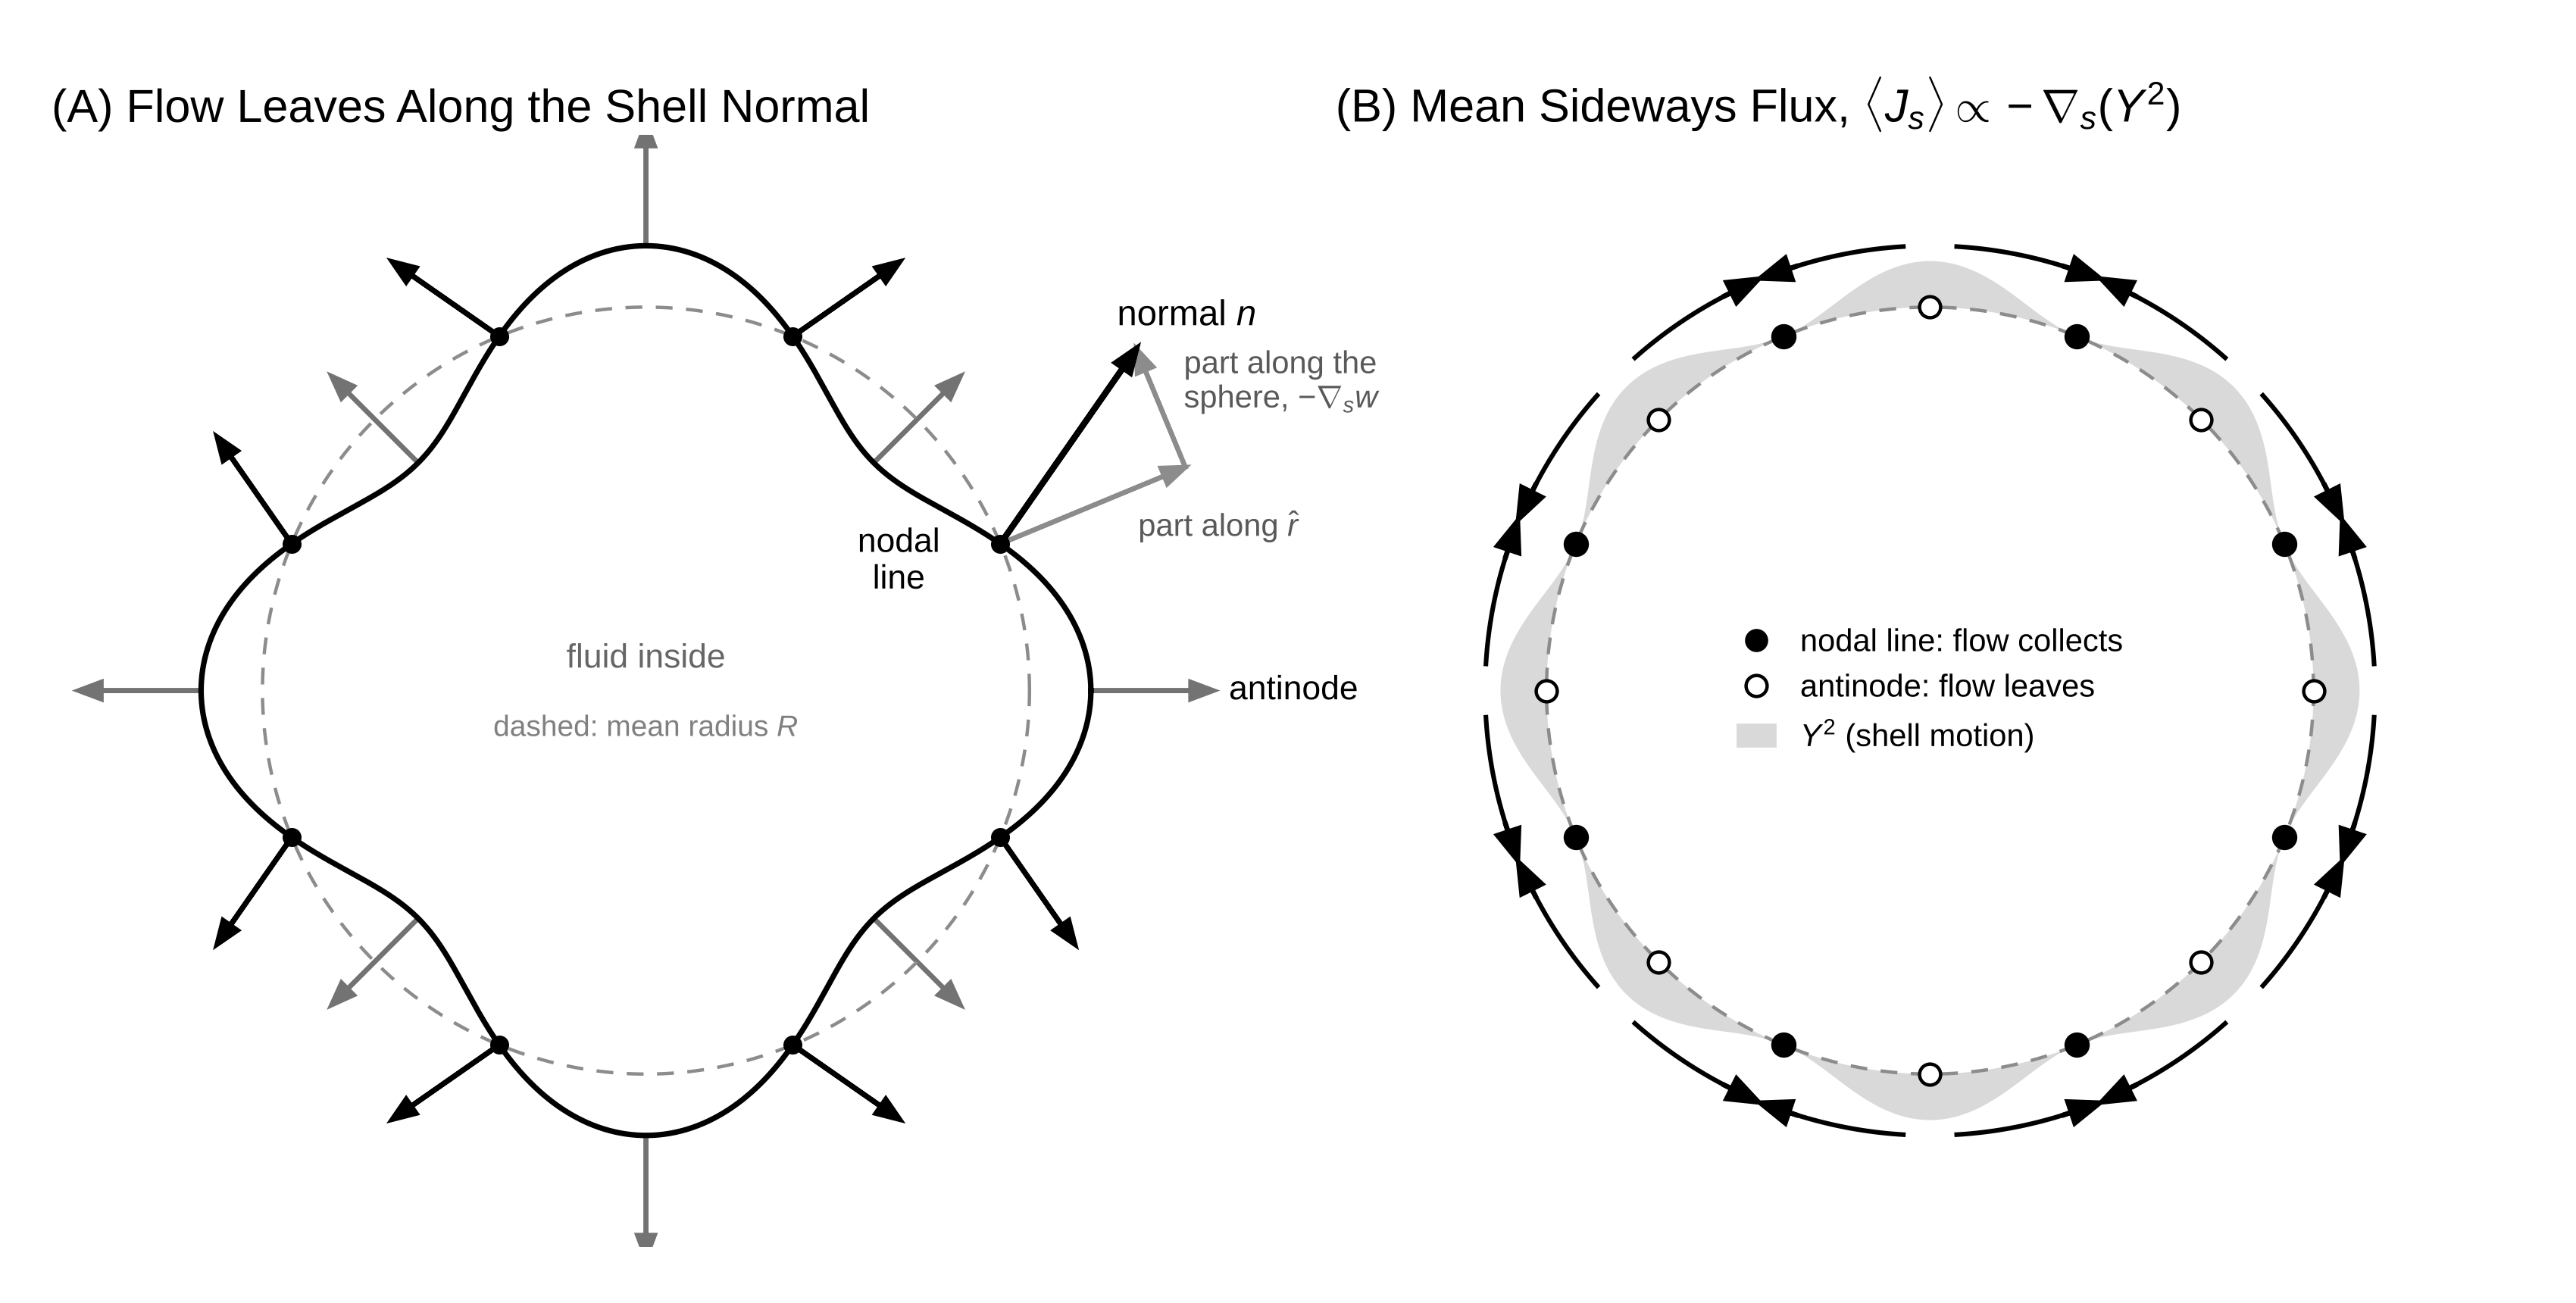
\includegraphics[width=\linewidth]{Figures/shell_flux_sketch.png}
\caption{Flow through a permeable vibrating shell, seen in a slice through its center. The shell vibrates in a standing mode $w = W_0\cos(\omega t)\,Y$, here with $Y = \cos 4\theta$ in the slice, and the vibration is drawn larger than scale. (A) The shell (solid) and its mean radius $R$ (dashed). Arrows show the outward normal $\bm{n} = \hat{\bm r} - \nabla_s w$, the direction in which fluid leaves the shell. At the antinodes (grey arrows) the shell is flat, and the normal points along the mean radius. At the nodal lines (black dots and arrows) the slope of the shell is largest, and the normal leans sideways. At one nodal line the normal is split into its part along the mean radius, $\hat{\bm r}$, and its part along the sphere, $-\nabla_s w$. (B) The sideways flux averaged over one cycle, $\langle \bm{J}_s \rangle \propto -\nabla_s(Y^2)$, for $k > 0$. The grey band shows $Y^2$, which is largest where the shell moves most. The flux runs from each antinode (open circles) toward the two nearest nodal lines (black dots), where the fluid collects.}
\label{fig:shell_flux}
\end{figure}

\section*{The Navier--Stokes Equations}

\paragraph{Conservation of Mass.} Let fluid be created inside the shell at the rate $\sigma$ per unit volume, so that $s = -\sigma$. With $\phi = \rho$ in Eq.~(\ref{eq:continuity}) and a constant density $\rho$,
%
\begin{equation}
\nabla\cdot\bm{u} = \frac{\sigma}{\rho}.
\label{eq:mass}
\end{equation}
%
Away from the source the velocity field has no divergence, $\nabla\cdot\bm{u} = 0$, which is the incompressibility condition.

\paragraph{Momentum Equation.} Newton's second law for the fluid follows from the same balance with $\phi = \rho\bm{u}$. Let $\bm{f}$ be an external force per unit volume, such as gravity, let $P$ be the stress tensor, and let the created fluid start at rest. Then
%
\begin{equation}
\frac{\partial (\rho \bm{u})}{\partial t} + \nabla \cdot (\rho \bm{u}\bm{u}) = -\nabla\cdot P + \bm{f}.
\end{equation}
%
The product rule gives $\partial(\rho\bm{u})/\partial t = \bm{u}\,\partial\rho/\partial t + \rho\,\partial\bm{u}/\partial t$ and $\nabla\cdot(\rho\bm{u}\bm{u}) = \bm{u}\,\nabla\cdot(\rho\bm{u}) + \rho\,(\bm{u}\cdot\nabla)\bm{u}$. By conservation of mass, $\partial\rho/\partial t + \nabla\cdot(\rho\bm{u}) = \sigma$, so
%
\begin{equation}
\rho\left(\frac{\partial \bm{u}}{\partial t} + \bm{u}\cdot\nabla\bm{u}\right) = -\nabla\cdot P + \bm{f} - \sigma\,\bm{u}.
\end{equation}
%
The last term is the force needed to bring newly created fluid up to the speed of the flow around it.

\paragraph{Stress Tensor.} The stress has two parts. The pressure $p$ pushes equally in all directions. Viscous stress resists the sliding of neighboring layers of fluid and, for small velocity gradients, grows in proportion to them. For a fluid with viscosity $\eta$,
%
\begin{equation}
P = p\,\mathbf{I} - \eta\left(\nabla\bm{u} + \nabla\bm{u}^{\mathsf T}\right) + \frac{2\eta}{3}\left(\nabla\cdot\bm{u}\right)\mathbf{I},
\end{equation}
%
where $\mathbf{I}$ is the identity tensor, so that $\nabla\cdot P = \nabla p - \eta\nabla^2\bm{u} - \tfrac{\eta}{3}\nabla(\nabla\cdot\bm{u})$. The Navier--Stokes equation with a source and a forcing term is then
%
\begin{equation}
\rho\left(\frac{\partial\bm{u}}{\partial t} + \bm{u}\cdot\nabla\bm{u}\right) = -\nabla p + \eta\nabla^2\bm{u} + \frac{\eta}{3\rho}\nabla\sigma + \bm{f} - \sigma\,\bm{u},
\label{eq:ns}
\end{equation}
%
where the Laplacian acts on each component of $\bm{u}$, $\nabla^2\bm{u} = \partial^2\bm{u}/\partial x^2 + \partial^2\bm{u}/\partial y^2 + \partial^2\bm{u}/\partial z^2$. Away from the source $\sigma = 0$, and the equation reduces to the ordinary Navier--Stokes equation with a body force.

\section*{Navier--Stokes Equations Inside a Vibrating Shell}

\paragraph{Conditions at the Shell.} Inside the fluid the Navier--Stokes equation holds unchanged. The shell enters through four conditions at its surface, applied at $r = R$ for small displacements. First, fluid crosses the shell as in Eq.~(\ref{eq:normal_bc}). Second, the fluid does not slide along the shell. Third, the rate of flow through the shell follows Eq.~(\ref{eq:permeation}). Fourth, the fluid pushes back on the shell, which moves under its own tension $T$, the normal stress of the fluid and the drive $f_d$,
%
\begin{equation}
\rho_s\,\frac{\partial^2 w}{\partial t^2} = \nabla_s\cdot\left(T\,\nabla_s w\right) + \left[\,p - 2\eta\,\frac{\partial u_r}{\partial r}\,\right]_{\rm in} - p_{\rm out} + f_d,
\label{eq:shell}
\end{equation}
%
where $\rho_s$ is the mass per unit area of the shell. The fluid and the shell thus form one coupled system: the shell sets the flow at the boundary, and the flow loads the shell.

\paragraph{Frame of the Shell.} The boundary of the fluid moves, which is awkward for calculation. A frame that stretches with the shell holds the boundary fixed. Let each point of the fluid move with the frame velocity $\bm{u}_m = (r/R)\,(\partial w/\partial t)\,\hat{\bm r}$, which matches the shell at $r = R$ and is zero at the center. A time derivative taken at a fixed point of this frame differs from one taken at a fixed point in space by $(\bm{u}_m\cdot\nabla)\bm{u}$, so away from the source Eq.~(\ref{eq:ns}) becomes
%
\begin{equation}
\rho\left(\frac{\partial \bm{u}}{\partial t}\bigg|_{\rm frame} + (\bm{u} - \bm{u}_m)\cdot\nabla\bm{u}\right) = -\nabla p + \eta\nabla^2\bm{u} + \bm{f}.
\end{equation}
%
The fluid is carried by its velocity relative to the vibrating frame. Near the shell the frame is still on the nodal lines and moves most at the antinodes.

\paragraph{Net Outflow.} Integrating Eq.~(\ref{eq:mass}) over the fluid inside the shell and applying the divergence theorem with Eq.~(\ref{eq:normal_bc}) gives
%
\begin{equation}
Q_{\rm out}(t) = \oint_{\rm shell}\left(\frac{\partial w}{\partial t} + q\right) dA = \int_{\Omega} \frac{\sigma}{\rho}\, dV \equiv Q_0,
\label{eq:outflow}
\end{equation}
%
where $Q_0$ is the volume of fluid created per unit time. The shell lets out fluid at the rate the source creates it, at every instant. The vibration adds nothing to this total. A constant displacement solves Eq.~(\ref{eq:shell}) with zero frequency, every vibrating mode is orthogonal to it, and so $\oint Y\, dA = 0$. The motion of the shell carries as much fluid in through some patches as it carries out through others. Without a source the net outflow is zero, and the vibrating shell conserves mass in the same way as the fixed control volume of the classical derivation.

\paragraph{Where the Fluid Leaves.} The vibration does not change how much fluid leaves, but it changes where the fluid leaves. The steady part of the flow, $q_0 = Q_0/(4\pi R^2)$, leaves evenly over the shell along the mean radius. The part $k\,w$ leaves through the patches between nodal lines in turn. When an antinode reaches its peak, the shell there is still and flat, and fluid leaves straight outward at the rate $q_0 + k\,W_0\,Y_{\max}$. Half a cycle later the same patch is at its trough and lets fluid out at the reduced rate $q_0 - k\,W_0\,Y_{\max}$. The steady part does not contribute to the mean sideways flux, since the slope averages to zero over one cycle, so Eq.~(\ref{eq:sideways}) holds with a source as well. The steady outflow is spread evenly over the shell, while the vibration steers the oscillating part along the sphere toward the nodal lines for $k > 0$. A tension gradient on the shell moves the nodal lines, and with them the lines along which the outflow gathers.

\paragraph{Mean Flow Driven by the Vibration.} For a small vibration of size $\epsilon$, write $\bm{u} = \epsilon\,\bm{u}_1 + \epsilon^2\,\bm{u}_2$ and $p = \epsilon\,p_1 + \epsilon^2\,p_2$, without a source or body force. At first order the flow oscillates with the shell and obeys the linear equation $\rho\,\partial_t\bm{u}_1 = -\nabla p_1 + \eta\nabla^2\bm{u}_1$, with $u_{1,r} = \partial_t w + k\,w$ and no sliding at $r = R$. At second order the average over one cycle, written $\langle\,\cdot\,\rangle$, gives a steady flow,
%
\begin{equation}
\eta\,\nabla^2\langle\bm{u}_2\rangle - \nabla\langle p_2\rangle = \rho\,\big\langle(\bm{u}_1\cdot\nabla)\bm{u}_1\big\rangle, \qquad \nabla\cdot\langle\bm{u}_2\rangle = 0.
\end{equation}
%
Moving the no-slip condition from $r = R + w$ to $r = R$ and keeping the terms of second order gives the mean flow along the sphere at the shell,
%
\begin{equation}
\langle\bm{u}_{2,s}\rangle = -\Big\langle w\,\frac{\partial \bm{u}_{1,s}}{\partial r}\Big\rangle - \big\langle u_{1,r}\,\nabla_s w\big\rangle = -\Big\langle w\,\frac{\partial \bm{u}_{1,s}}{\partial r}\Big\rangle - \frac{k\,W_0^2}{4}\,\nabla_s\big(Y^2\big).
\end{equation}
%
The second term is the sideways flux of Eq.~(\ref{eq:sideways}), found here from the momentum equation. The first term comes from the thin layer of fluid that the shell drags back and forth. Together they set a mean flow along the shell toward or away from the nodal lines, and this flow drives a steady circulation inside the shell.

\end{document}
